\documentclass[11pt]{article}
%-----------Packeges---------------%
\usepackage{amsmath}
\usepackage{amssymb}
\usepackage{amsfonts}
\usepackage{tocloft}
\usepackage{float}
\usepackage{graphicx}
\usepackage[bookmarks=true]{hyperref}
\usepackage{fancyhdr}


%----------Definition & Theorem----%
\newtheorem{definition}{Definition}[subsection]
\newtheorem{theorem}{Theorem}[subsection]
\newtheorem{proposition}{Proposition}[subsection]
\newtheorem{lemma}{Lemma}[subsection]
\newtheorem{corollary}{Corollary}[subsection]

\pagestyle{fancy}
\fancyhead[L]{Math 417}
\fancyhead[C]{HW7}
\fancyhead[R]{Lanxiao Bai(lbai5)}
\begin{document}
	\paragraph{2.5.7}
		\textbf{Claim:} For a subgroup $N$ of a group $G$, the following are equivalent:
		\begin{enumerate}
			\item $N$ is normal
			\item $\forall a \in G, \exists b \in G, aN = Nb$.
			\item $\forall a \in G, aN = Na$.
		\end{enumerate}
		
		\textbf{Proof:} To prove all three statements are equivalent to each other, we can prove that $1 \Rightarrow 2, 2 \Rightarrow 3 $ and $3 \Rightarrow 1$.
		
		$1 \Rightarrow 2$:
		
			Since $N$ is normal, we know $\forall g \in G, gNg^{-1} = N$ by definition. 
			
			Then, we have $\forall g \in G, gN = Ng$, which means $b = a$.
			
		$2 \Rightarrow 3$:
			
			Since $\forall a \in G, \exists b \in G, aN = Nb$, and $aN$ is a coset of $N$, we know it's either $a \in aN = bN = Nb$ or $aN \cap bN = \emptyset$. Since $aN = Nb$, $b \in Nb = aN$, so the second possibility is ruled out. Thus, we have $bN = Nb$ for all $b \in G$ which is equivalent to $aN = Na$ for all $a \in G$.
		
		$3 \Rightarrow 1$:
		
			Since $\forall a \in G, aN = Na$, we can get $aNa^{-1} = N$ by multiply $a^{-1}$ on both sides, which means $N$ is normal.
			
			As a result, we can conclude that all three statements are equivalent.$\blacksquare$ 
	\paragraph{2.5.13}
		\subparagraph{(a)}
			\textbf{Claim:} The center of group $G$ is a normal subgroup of $G$.\\
			
			\textbf{Proof:}
			Since $\mathrm{Center}(G) = \{x | \forall g \in G, gx = xg\}$, we have $\mathrm{Center}(G) = {x | gxg^{-1} = x}$ which is exactly the definition of normal subgroup.$\blacksquare$
		\subparagraph{(b)}Based on the multiplication table of $S_3$:
		\begin{figure}[H]
        	\begin{center}
        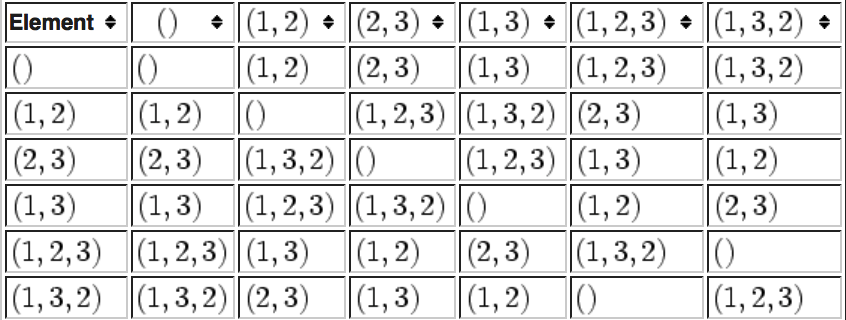
\includegraphics[width=8cm]{./imgs/S_3.png}
        	\caption{$S_3$}
        	\end{center}
    	\end{figure}

			\[\mathrm{Center}(S_3) = \{e\}\]
	\paragraph{2.6.1}
		\subparagraph{Claim:} Relation defined on $X$ by $x_1 \sim x_2$ if $f(x_1) = f(x_2)$ is an equivalence relation. And the associated partition of X is the partition into $f^{-1}(y)$ for $y \in Y$.
		
		\subparagraph{Proof:} We can prove the relation is equivalent relation first by proving its reflexivity, symmetry and transitivity.
		
		\textbf{Reflexivity:} $\forall x \in X$, it's obvious that $x = x$ and $f(x) = f(x)$, so $x \sim x$.
		
		\textbf{Symmetry:} Take 2 arbitrary $x, y \in X$, then if $x \sim y$, $x = y \Rightarrow f(x) = f(y) = f(y) = f(x) \Rightarrow y \sim x$. So we have $x \sim y \Leftrightarrow y \sim x$.
		
		\textbf{Transitivity:} Take $x, y, z \in X$. If $x \sim y$ and $y \sim z$, then $x = y \Rightarrow f(x) = f(y)$ and $y = z \Rightarrow f(y) = f(z)$. So $x = y = z \Rightarrow f(x) = f(y) = f(z)$, which means $x \sim z$.
		
		So we proved this relation is an equivalent relation.
		
		Then we can prove the associated partition of X is the partition into fiber.
		
		Since $f$ is a surjective, $\forall y \in Y, \exists x \in X$ that $f^{-1}(y) = x$. And as we have an equivalent relation on $X$, each $x \in X$ is and only is in one equivalent class is guaranteed by the correspondent partition of $X$. So each subsets of $f^{-1}$ are disjoint. And since we know $f$ is a injection by the definition of the relation, $f$ and $f^{-1}$ are bijections. Thus, $X = f^{-1}(Y)$, so the partition into fibers is exactly the partition of $X$.$\blacksquare$
		
	\paragraph{2.7.9}
		\subparagraph{Claim:} The commutator subgroup $C$ of group $G$ is normal. And quotient group $G / C$ is abelian. If $H \unlhd G$ and $G /H$ is abelian, then $C \subseteq H$. 
		
		\subparagraph{Proof:} Let $a, b \in G$ and $x = gag^{-1}, y = gbg^{-1}, x^{-1} = ga^{-1}g^{-1}, y^{-1} = gb^{-1}g^{-1}$. Then take $c = xyx^{-1}y^{-1} \in C$, $gcg^{-1} = aba^{-1}b^{-1} \in C \Rightarrow gCg^{-1} = C$.
		
		Thus, $C$ is a normal group.
		
		Take $a, b \in C$, so $aC, bC, Ca, Cb \in  G / C$. Since $C$ is normal as we've proved, $aCbC = abC = Cab$. To prove $G / H$ is abelian, we want to prove that $Cab = Cba$ for all $a, b \in G$. Since we know $Cab$ and $Cba$ are both right cosets of $C$, so it's either they are equal, or they are disjoint. Let $b = x = y = e$, we have $a \in Cab$ and $a \in Cba$, so they can't be disjoint.
		
		 As a result, $Cab = Cba$, and $G / C$ is abelian by definition.
		 
		 Since $H$ is normal and $G /H$ is abelian, take arbitrary $c \in C$, as implied in the first part and second part of the proof, $gcg^{-1} = aba^{-1}b^{-1} \in C, Cab = Cba \Rightarrow c \in H$. 
		 
		 Thus, $C \subseteq H$ by definition.$\blacksquare$ 
		 
		 
		
\end{document}
